%\begin{sidewaysfigure}
%  \begin{center}
%  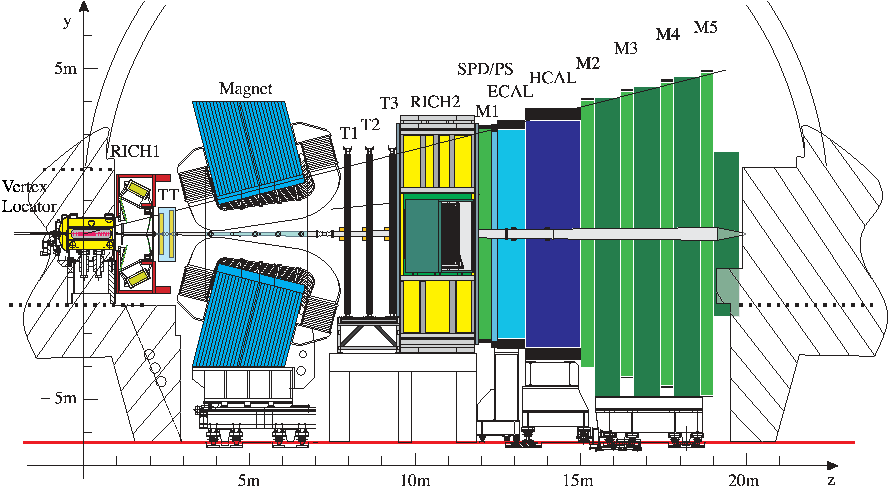
\includegraphics[width=0.8\textheight]{lhcb-detector-cross-section}
%  \caption[Cross-section view of \LHCb, cut in the non-bending $y$--$z$ plane]%
%    {Cross-section view of \LHCb, cut in the non-bending $y$--$z$ plane.}
%  \label{fig:LHCbCrossSection}
%  \end{center}
%\end{sidewaysfigure}



\chapter{Selection of neutrino interactions in the ECal}
\label{chap:NeutrinoInteractionSelection}
This analysis presents a measurement of the CC inclusive interaction cross-section of $\nu_\mu$ with lead nuclei using the ND280 tracker ECals.  To make such a measurement, a sample of neutrino interaction vertices within the ECal must be found.  The selection of events is based on the enhanced reconstruction outlined in chapter~\ref{chap:EnhancedECalReconstruction}.  However, as described in section~\ref{sec:ReconOutput}, the output of the enhanced reconstruction has been kept generic and isn't specifically tailored to this task.  The reconstruction's outputs a set of clusters which contain a set of 3D tracks and every pairwise crossing that said tracks make.  While it is true that is some situations the reconstruction will accurately represent a vertex out of the box, e.g. when only two tracks are reconstructed in the cluster, there will be many situations where extra reconstruction steps are needed before any further selection can take place.

%\section{Data selection}
%Data flags

\section{Monte Carlo selection}
Make the cuts

\section{Properties of events in selection}

